\documentclass[12pt]{article}
\usepackage{amssymb, amsmath, hyperref}
\DeclareMathAlphabet{\mathscr}{OT1}{pzc}{m}{it}
\usepackage{epsfig,float, setspace, graphicx, setspace, wrapfig, subfig}
\usepackage{verbatim}
\usepackage{fullpage,setspace}
\title{Photon-Bunching in Quantum Memory}
\author{Adam A. S. Green\\University of Calgary}
\begin{document}
\bibliographystyle{plain}
\maketitle
\section{Introduction}

There is a simple analogy between a beamsplitter and a quantum memory. If one thinks of a beamsplitter as two distinct modes, $a$ and $b$, the action of the beamsplitter is to mix these modes in a certain way. For instance, a 50-50 beamsplitter means that a single photon in mode $a$ will have a 50$\%$ chance of staying in mode $a$ and a 50\% of becoming mode $b$.

In the same way, a quantum memory deals with two modes: photon and atomic excitation. The action of the quantum memory will be to mix the two modes in a certain way. Usually, one wants to completely convert the photon mode into an atomic mode, or vis versa. However, if one used a 50\% efficient quantum memory, we obtain a very similar situation as that of a beamsplitter.

This is interesting, as there is a phenomena that occurs in beamsplitters called `photon-bunching', where--due to the boson statistics-- if you have a photon incident on the beamsplitter in mode $a$, and another photon incident in mode $b$, you have a 50\% chance of seeing two photons in mode $a$, and a 50\% chance of seeing two photons in mode $b$. 

The purpose of this report is to quantify and illustrate the extent of similarities between a beamsplitter and a quantum memory.
\doublespacing
\section{CD Memory}
We can demonstrate photon bunching explicitly in the case of the CD memory\cite{arxiv}. This quantum memory is used because the author was familiar with the equations of motion.

We have previously derived the Heisenberg equations of motion for the operators of interest, $E_{\textrm{out}}$ and $\sigma_{\textrm{z?}}$.

The heisenburg state we prepared for photon bunching is:
\begin{equation}
| \Psi \rangle = \sigma(t=0)^\dagger \int d\omega \psi(w) E_0^\dagger(w) | 0 \rangle
\end{equation}

Where $E_0(\omega)$ is the creation operator of a photon of frequency $\omega$, $\psi(\omega)$ is the single-photon envelope in frequency space, and $\sigma(t=0)$ is the initial creation operator of a atomic excitation. In what follows, we will be assuming that a photon is already stored in the memory at $t=0$, and that another pulse is incident.

The three terms we are concerned with are:
\begin{align}
\langle \psi_{20}| \Psi \rangle &=\langle 0 | \frac{1}{\sqrt{2}}\sigma (t)\sigma(t) | \Psi \rangle\\
\langle \psi_{11} | \Psi \rangle& =\langle 0 |  \sigma(t') \int^{t'} dt E_\textrm{out}(t) | \Psi \rangle\\
\langle \psi_{02} | \Psi \rangle &= \langle 0 |  \frac{1}{\sqrt{2}}\int dt \int dt' E_\textrm{out}(t) E_\textrm{out}(t') | \Psi \rangle
\end{align}

Where $| \psi_{20} \rangle$ is a double excitation in the photon field, $| \psi_{11} \rangle $ is photon and an atomic excitation, and $ | \psi_{02} \rangle $ is a double atomic excitation. 
\section{$| \psi_{11} \rangle$}
First, we consider the term that deals with a single excitation in the field and a single
excitation in the atom. If photon-bunching is seen in this memory, then this term should
equal zero.

\begin{align}
\left | \langle \psi_{11} | \Phi \rangle \right | ^2 &=\int^{t'} dt \left | \langle 0 | E_\textrm{out}(t) \sigma(t') \int d \omega \phi(\omega)E^\dagger_0(\omega)
\sigma^\dagger(0) | 0 \rangle \right |^2 \\
\end{align}

Physically (in terms of detectors), the above equation corresponds to having two measurements.
In the first, you are directly measuring the atomic ensemble at time $t=t'$.
In the second, you have left a photon detector on to measure the resaviour field from time $t={-\infty,t'}$.
Concisely, this measures the probability of both: seeing a photon in the resovior field, and seeing an atomic excitation.


We also know the equations for $E_\text{out} (t)$ and $\sigma (t)$ from our previous work.

\begin{align}
E_\textrm{out}(t) &= E_\textrm{in}(t) + i \sqrt{\frac{2}{\kappa}} g(t) \sigma(t)\\
\sigma(t) &= \sigma(0) e^{-\tau} + i\sqrt{2} e^{-\tau} \int^\tau_w d t' e^\tau E_\textrm{in}(t) \frac{g(t)}{\sqrt{\kappa}}
\end{align}
Where $\tau = \int^t dt g^2(t)/\kappa$, $g(t)$ is a time-dependant coupling between the atomic ensemble and the cavity field, and $\kappa$ is the decay rate of the cavity. Inserting these equations we obtain:
\begin{align}
\left | \langle \psi_{11} | \Phi \rangle \right | ^2 &= \int^{t'} dt \left | \langle 0 |
   \left(  E_\textrm{in}(t) + i \sqrt{\frac{2}{\kappa}} g(t) \sigma(t) \right ) \times \right.\\
   &\left. \qquad \qquad \left (\sigma(0) e^{-\tau} + i\sqrt{2} e^{-\tau} \int^\tau_w d t' e^\tau E_\textrm{in}(t) \frac{g(t)}{\sqrt{\kappa}}\right)|\Psi \rangle \right |^2\\
\end{align}

Expanding this out, we get the following terms:
\begin{align}
\left | \langle \psi_{11} | \Phi \rangle \right | ^2 &= 
\int^{t'} dt \left | \langle 0 | E_\textrm{in}(t) \left( \sigma(0) e^{-\tau(t')} + i\sqrt{2} e^{-\tau(t')} \int^{t'} d t'' e^{\tau(t'')} E_\textrm{in}(t'') \frac{g(t'')}{\sqrt{\kappa}} \right )\right. \\
&\qquad+ i \sqrt{\frac{2}{\kappa}}g(t)\left (\sigma(0) e^{-\tau} + i\sqrt{2} e^{-\tau} \int^{t}d t''' e^{\tau(t''')} E_\textrm{in}(t''') \frac{g(t''')}{\sqrt{\kappa}} \right) \times\\
&\left.\qquad \left(\sigma(0) e^{-\tau(t')} + i\sqrt{2} e^{-\tau(t')} \int^{t'} d t'' e^\tau(t'') E_\textrm{in}(t'') \frac{g(t'')}{\sqrt{\kappa}}\right) | \Psi \rangle \right |^2 
\end{align}

If we apply the commutation relations, we can get rid of any terms that don't have $E_\textrm{in}(t)$ and $\sigma(0)$ in them, as any term in the above equation that doesn't have both of these operators will be annihilated through simple commutations. Ie. if a term only has $E_\textrm{in} E_\textrm{in}$, we know that $|\Psi\rangle$ contains a $\sigma^\dagger(0)$, and that $\sigma^\dagger(0)$ and $E_\textrm{in}$ commute, so $\sigma^\dagger(0)$ can move through and act as $\langle 0 | \sigma^\dagger(0) = 0$. So any term that survives must contain terms that don't commute with $E_\textrm{in}$ as well as $\sigma(0)$.

This leaves us with the following terms:
\begin{align}
\left | \langle \psi_{11} | \Phi \rangle \right | ^2 &= \int^{t'} dt \left | \langle 0 | E_\textrm{in}(t) \sigma(0) e^{-\tau(t')}
\sigma^\dagger(0) \int d\omega E_0(\omega) \phi(\omega) | 0 \rangle -\right. \\
&\qquad  \langle 0 | \frac{2}{\sqrt{\kappa}} g(t) \sigma(0) e^{-\tau(t) -\tau(t')}
\int^{t'} dt'' e^{\tau(t'')} E_\textrm{in}(t'')\frac{g(t'')}{\sqrt{\kappa}} \sigma^\dagger(0) \int d\omega E_0(\omega) \phi(\omega) | 0 \rangle - \\
& \qquad \left. \langle 0 | \frac{2}{\sqrt{\kappa}} g(t) \sigma(0) e^{-\tau(t) -\tau(t')}
\int^{t} dt''' e^{\tau(t''')} E_\textrm{in}(t''')\frac{g(t''')}{\sqrt{\kappa}} \sigma^\dagger(0) \int d\omega E_0(\omega) \phi(\omega) | 0 \rangle \right |^2
\end{align}


We know that $E_\textrm{in}$ is the input-pulse, and can also be defined in frequency space as $E_\textrm{in} = \int dw e^{-iwt} E_0(\omega) $ and furthermore, $[E_0(\omega), E_0^\dagger(\omega') ] = \delta(\omega-\omega')$, thus we know that 

\begin{align}
\langle 0 |E_\textrm{in}(t) \int d\omega \phi(\omega) E^\dagger_0(\omega) | 0 \rangle\\
&= \langle 0 | \int d \omega' \int d \omega E_0(\omega') E_0(\omega) \phi(\omega) e^{-i\omega t} |0\rangle\\
&=\int d \omega' \int d \omega \delta(\omega'-\omega) \phi(\omega) e^{-i\omega t}\\ 
&= \mathscr{F}\{\phi(\omega)\} \equiv \tilde{\phi}(t)
\end{align}

using this property, the equation reduces to:
%As well, if we make the simplifying assumption that $\tilde{\phi}(t) = \sqrt{\frac{2}{\kappa}} g(t)e^{\tau(t)}$, then %the equation reduces to:

\begin{align}
\left | \langle \psi_{11} | \Phi \rangle \right | ^2 &= \int^{t'} dt\left| \tilde{\phi}(t)e^{-\tau(t')} -\frac{2}{\sqrt{\kappa}} g(t) e^{-\tau(t)-\tau(t')} \int^{t'} \tilde{\phi}(t'')\frac{g(t'')}{\sqrt{\kappa}} dt'' - \right.\\
&\left. \qquad \frac{2}{\sqrt{\kappa}} g(t) e^{-\tau(t)-\tau(t')} \int^t \tilde{\phi}(t''')\frac{g(t''')}{\sqrt{\kappa}} dt''' \right |^2 
\end{align}

Note, we haven't shown how the $\sigma(0) \sigma^\dagger(0)$ term vanishes, but using the commutator properties, you can show that in this case you can simply replace this term with unity.

This is a completely general equation, as we have not assumed anything about the shape of the incoming field. 
To simply this equation however, we can make the assumption that the incoming field meets the optimal condition discussed
in the original paper.

This allows us to do two things. First, because the field is optimally conditioned, all of the efficiency is controlled by the value of $\tau_w$, so we only have one variable to deal with. Second, it will allow the above equation to be integrated very simply.

The optimal condition requires that: $\tilde{\phi}(t) = \sqrt{\frac{2}{\kappa}} g(t) e^{\tau(t)}$

However, we also have to normalize the incoming field, such that:
\begin{equation}
\int^\infty_\infty | \tilde{\phi}(t) |^2 dt' =1
\end{equation}

Plugging the optimal field condition in, the normalization condition reduces to:
\begin{align}
\int^\infty_\infty A^2| \tilde{\phi}(t) |^2 dt' &=1\\
\int^\infty_\infty A^2 \frac{2}{\kappa} g^2(t) e^{2\tau(t)} &=1\\
 A^2 \left( e^{2\tau_w} -1\right)&=1
 \end{align}
 Thus, the value of $\tau$ when $t=\infty$ defines the normalization constant. 
 \begin{equation}
 A = \sqrt{\frac{1}{\left(  e^{2\tau_w} -1\right)}}
 \end{equation}

 We can also note that in the specific case where $\eta = 1/2$, i.e. when the efficiency is one-half, then $\tau_w = \ln(\sqrt{2})$ and our normalization coefficient becomes:
 \begin{align}
 A &= \sqrt{\frac{1}{\left(  e^{2\ln(\sqrt{2})} -1\right)}}\\
 A &= \sqrt{\frac{1}{\left( 2-1 \right ) }}\\
 A &= 1
 \end{align}
Inserting this into our equation, we obtain:

\begin{align}
\left | \langle \psi_{11} | \Phi \rangle \right | ^2 &= A^2\int^{t'} dt \left | \sqrt{\frac{2}{\kappa}} g(t) e^{\tau(t)-\tau(t')} \right.
      -2\sqrt{\frac{2}{\kappa}}g(t) e^{-\tau(t)-\tau(t')} \int^{t'} \frac{g(t'')^2}{\kappa} e^{2\tau(t'')} dt'' \\
       &\qquad \left.-2\sqrt{\frac{2}{\kappa}} g(t) e^{\tau(t')-\tau(t)} \int^t \frac{g(t''')^2}{\kappa} e^{2\tau(t''')} dt'''\right |^2
\end{align}

and, knowing that $\frac{g^2(t)}{\kappa}dt = d\tau$, the above can be integrate to obtain:

\begin{align}
\left | \langle \psi_{11} | \Phi \rangle \right | ^2 &=A^2\int^{t'} dt \left| \sqrt{\frac{2}{\kappa}} g(t) e^{\tau(t)-\tau(t')} - \sqrt{\frac{2}{\kappa}} g(t)\left( e^{\tau(t)-\tau(t')} - e^{-\tau(t')-\tau(t)} \right )\right.\\
&\left. \qquad -\sqrt{\frac{2}{\kappa}} g(t) \left( e^{\tau(t')-\tau(t)} - e^{-\tau(t')-\tau(t)} \right)\right|^2 
\end{align}

which can be factored to obtain:
\begin{align}
\label{p11}
\left | \langle \psi_{11} | \Phi \rangle \right | ^2  &= A^2\int^{t'} dt \left|\sqrt{\frac{2}{\kappa}} g(t) e^{-\tau(t)} \left (- e^{\tau(t')} +2 e^{-\tau(t')} \right ) \right |^2 
\end{align}

If we use the condition that $\eta=0.5$, then $\tau(t') = \textrm{ln}(\sqrt{2})$. It should be noted that $\tau(t=\infty) = \tau(t')$. That is, we have let an infinite time pass when we do the measurement. We are preforming a measurement on the atomic ensemble at time $t'$, but we have left out photon detectors on from time $t_0$ to $t'$. However, because we know what $\tau(t')$ is equal to, we can evaluate the term in brackets in the above equation.

\begin{align}
\left | \langle \psi_{11} | \Phi \rangle \right | ^2 = A^2\int^{t'} dt \left| \sqrt{\frac{2}{\kappa}} g(t) e^{-\tau(t)} \left ( e^{\textrm{ln}(\sqrt{2})} -2 \frac{1}{e^{\textrm{ln}({\sqrt{2}})}} \right ) \right|^2 = 0 
\end{align}

This shows that there is zero chance to measure a photon in the reservoir field and an atomic excitation when the quantum is operating at $50\%$ efficiency. This is precisely what is expected for a beam-splitter.


\section{ $| \psi_{20} \rangle$}
Next, we deal with the case term that measures the amplitude of obtaining a double excitation in the atomic ensemble.
\begin{align}
\langle \psi_{20}| \Psi \rangle &=\langle 0 |\frac{1}{\sqrt{2}} \sigma(t)\sigma (t)| \Psi \rangle\\
\langle \psi_{20}| \Psi \rangle &=\langle 0 | \frac{1}{\sqrt{2}} \sigma \sigma 
\sigma(t=0)^\dagger \int d\omega \psi(w) E_0^\dagger(w) | 0 \rangle
\end{align}

and the heisenburg equations for the operators $E_\textrm{out}$ and $\sigma$ are:
\begin{align}
E_\textrm{out}(t) &= E_\textrm{in}(t) + i \sqrt{\frac{2}{\kappa}} g(t) \sigma(t) \\
\sigma(t) &= \sigma(0) e^{-\tau} + i\sqrt{2} e^{-\tau} \int^{t_w} d t' e^\tau E_\textrm{in}(t) \frac{g(t)}{\sqrt{\kappa}}
\end{align}
Where $\tau = \int^t dt g^2(t)/\kappa$, and $g(t)$ is a time-dependant coupling between the atomic ensemble and the cavity field, and $\kappa$ is the decay rate of the cavity. Inserting these equations we obtain:
\begin{multline}
\langle \phi_{20}| \Psi \rangle =\langle 0 | \frac{1}{\sqrt{2}} \left (  \sigma(0) e^{-\tau} + i\sqrt{2} e^{-\tau} \int^{t_w} d t' e^\tau E_\textrm{in}(t) \frac{g(t)}{\sqrt{\kappa}} \right )\\ \left ( \sigma(0) e^{-\tau} + i\sqrt{2} e^{-\tau} \int^{t_w} d t' e^\tau E_\textrm{in}(t) \frac{g(t)}{\sqrt{\kappa}} \right ) \sigma(t=0)^\dagger \int d\omega \psi(w) E_0^\dagger(w) | 0 \rangle
\end{multline}
As shown before, we know the following relation,
\begin{equation}
E_\textrm{in} \int dw' \phi(\omega') E_0^\dagger(\omega') = \mathscr{F}[\phi(\omega)]
\end{equation}

And we know that the only terms that will survive in $\langle \phi |$ must contain $E_\textrm{in}(t) \sigma(t)$. This leaves the following expansion:
\begin{align}
\langle \psi_{20}| \Psi \rangle &= 2 i e^{-2\tau} \sigma(0) 
\int^{t} E_{in}(t') \frac{g(t')}{\sqrt{\kappa}} e^{\tau'} \sigma^\dagger(0) \int dw' E_0^\dagger(\omega') \phi(\omega')\\ 
&= 2 i e^{-2 \tau} \int d \tau' e^{\tau'} 
 \mathscr{F}(\phi(\omega)) \frac{\sqrt{\kappa}}{g(\tau')}
\end{align}

Now, we can also make a simplifying assumption, by noting that the optimal read-in condition is met when $\mathscr{F}(\psi(\omega)) =A \sqrt{\frac{2}{\kappa}} g(t) e^{\tau(t)}$ and under this condition is met, the above equation reduces to:
\begin{align}
\langle \psi_{20}| \Psi \rangle & =A 2\sqrt{2} i e^{-2\tau} \int d \tau' e^{2 \tau} \\
& =A \sqrt{2} i\left(1- e^{-2\tau}\right)
\end{align}
With the probability equal to:
\begin{align}
\label{p20}
|\langle \psi_{20}| \Psi \rangle|^2 &=|A 2\sqrt{2} i e^{-2\tau} \int d \tau' e^{2 \tau'}|^2 \\
&= |A  \sqrt{2} i (1-e^{-2\tau_w})|^2
\end{align}
Also, as previously shown, we know that $\tau_w$ is equal to $\tau_w = \ln{\sqrt{2}}$, so we can evaluate the above equation to obtain (remembering that $A = 1$:
\begin{align}
|\langle \psi_{20}| \Psi \rangle|^2 &= |\sqrt{2} i \frac{1}{2}|^2 \\
&= \frac{1}{2}
\end{align}

\section{$| \psi_{02} \rangle $}

We could invoke a conservation of probability to show that since this is the only other state that is possible in the double excitation space, it must have probability $1/2$, however it is good to do the calculations out to double check.

The quantity that we are interested in is the probability of measuring a double excitation in the reservoir field:

\begin{align}
|\langle \psi_{02} | \Psi \rangle |^2 =\int dt \int dt' \left | \langle 0 |\frac{1}{\sqrt{2}} E_\textrm{out}(t) E_\textrm{out}(t') \sigma^\dagger(0) \int d \omega \phi(\omega) E_0(\omega) | 0 \rangle \right |^2
\end{align}

Using the equations for $E_\textrm{out}(t)$, this becomes:
\begin{align}
\left | \langle \psi_{02} | \Phi \rangle \right | ^2 & =\int dt \int dt'\left |  \frac{1}{\sqrt{2}}\left ( E_\textrm{in}(t) 
+ i \sqrt{\frac{2}{\kappa}} g(t)\left ( \sigma(0) e^{-\tau} +
i\sqrt{2} e^{-\tau} \int^t d t''' e^\tau(t''') E_\textrm{in}(t''') \frac{g(t''')}{\sqrt{\kappa}} \right ) \right) \right .\times \\
 &\qquad \left. \left (E_\textrm{in}(t') + i \sqrt{\frac{2}{\kappa}} g(t')\left( \sigma(0) e^{-\tau(t')} +
 i\sqrt{2} e^{-\tau(t')} \int^{t'} d t'' e^\tau(t'') E_\textrm{in}(t'') \frac{g(t'')}{\sqrt{\kappa}}\right ) \right )  \Psi \rangle \right |^2
\end{align}

 
 As before, we know that only terms that contain $E_\textrm{in}$ and $\sigma(0)$ will survive the expansion. With this in 
 mind, we can reduce the above equation to:
\begin{align}
 \left | \langle \psi_{02} | \Phi \rangle \right | ^2 & = \frac{1}{2}\int dt \int dt'\left |\langle 0 | E_\textrm{in}(t) i \sqrt{\frac{2}{\kappa}} g(t') e^{-\tau(t')}\sigma(0) + E_\textrm{in}(t') i \sqrt{\frac{2}{\kappa}} g(t) e^{-\tau(t)}\sigma(0) +\right.\\
&\qquad -i\sqrt{2}\frac{2}{\sqrt{\kappa}}g(t')g(t) e^{-\tau(t')-\tau(t)}\sigma(0) \int ^{t'} dt'' E_\textrm{in}(t'')\frac{g(t'')}{\sqrt{\kappa}} e^{\tau(t'')}\\
&\qquad \left. -i\sqrt{2}\frac{2}{\sqrt{\kappa}}g(t')g(t) e^{-\tau(t')-\tau(t)}\sigma(0) \int ^t dt''' E_\textrm{in}(t''')\frac{g(t''')}{\sqrt{\kappa}} e^{\tau(t''')}| \Psi \rangle \Psi \rangle\right |^2
 \end{align}
 
Again, knowing that


\begin{align}
\langle 0 |E_\textrm{in}(t) \int d\omega E^\dagger_0(\omega) | 0 \rangle= \mathscr{F}\{\phi(\omega)\} \equiv \tilde{\phi}(t)
\end{align}
and again using the optimization condition: $\tilde{\phi}(t) =A \sqrt{\frac{2}{\kappa}} g(t) e^{\tau}$, we can obtain the following equation:

\begin{align}
\left | \langle \psi_{02} | \Phi \rangle \right | ^2 & =A \frac{1}{2}\int dt \int dt'\left | \frac{2}{\kappa} i g(t) g(t') \left(e^{\tau-\tau'} +e^{-(\tau-\tau')}\right) -\right.\\
&\qquad \left.i \frac{4}{\kappa}g(t) g(t') e^{-\tau-\tau(t')}\left( \int^{t'} d \tau(t'') e^{2\tau(t'')} + \int^t d \tau(t''') e^{2\tau(t''')} \right) \right |^2
\end{align}

Integrating this, we obtain:
\begin{align}
\left | \langle \psi_{02} | \Phi \rangle \right | ^2 & =A^2 \frac{1}{2}\int dt \int dt'\left | \frac{2}{\kappa} i g(t) g(t') \left(e^{\tau-\tau'} +e^{-(\tau-\tau')}\right) -\right.\\
&\qquad \left.i \frac{2}{\kappa}g(t) g(t') e^{-\tau-\tau(t')}\left( e^{2\tau(t')}-1 - e^{2\tau(t)}-1 \right) \right |^2 \\
 &=A^2  \frac{1}{2}\int dt \int dt'\left | \frac{2}{\kappa} i g(t) g(t') \left(e^{\tau-\tau'} +e^{-(\tau-\tau')}\right) -\right.\\
&\qquad \left.i \frac{2}{\kappa}g(t) g(t') \left( e^{\tau(t')-\tau(t)} + e^{\tau(t)-\tau(t')}-2e^{-\tau(t)-\tau(t')} \right) \right |^2
\end{align}

There is some cancellation, leaving:

\begin{align}
\label{p02}
\left | \langle \psi_{02} | \Phi \rangle \right | ^2 & =A^2\int dt \int dt'\left |i 2\frac{\sqrt{2}}{\kappa} g(t)g(t') e^{-\tau(t)-\tau(t')} \right|^2 \\
&=A^2 \frac{8}{4} \left ( e^{-2\tau_w}-1\right)^2\\
\end{align}

Now, if we require that $\tau_w = \textrm{ln}(\sqrt{2})$, this further reduces to:
\begin{align}
\left | \langle \psi_{02} | \Phi \rangle \right | ^2 &=2(-\frac{1}{2})(-\frac{1}{2})=\frac{1}{2}
\end{align}

\section{Full-Equivalence}
We have shown that the CD memory behaves like a beamsplitter under the very specific condition that $\eta = 1/2$, however, this suggests that there may be some mapping whereupon the equations that describe the CD memory are exactly mapped to the equations that describe a beamsplitter. 

First, if we plot Equations \eqref{p11},\eqref{p02},\eqref{p20} (taking into account that the normalization factor $A$ is dependant on $\tau(t=\infty)$), then we obtain the following graph:
\begin{figure}[H]
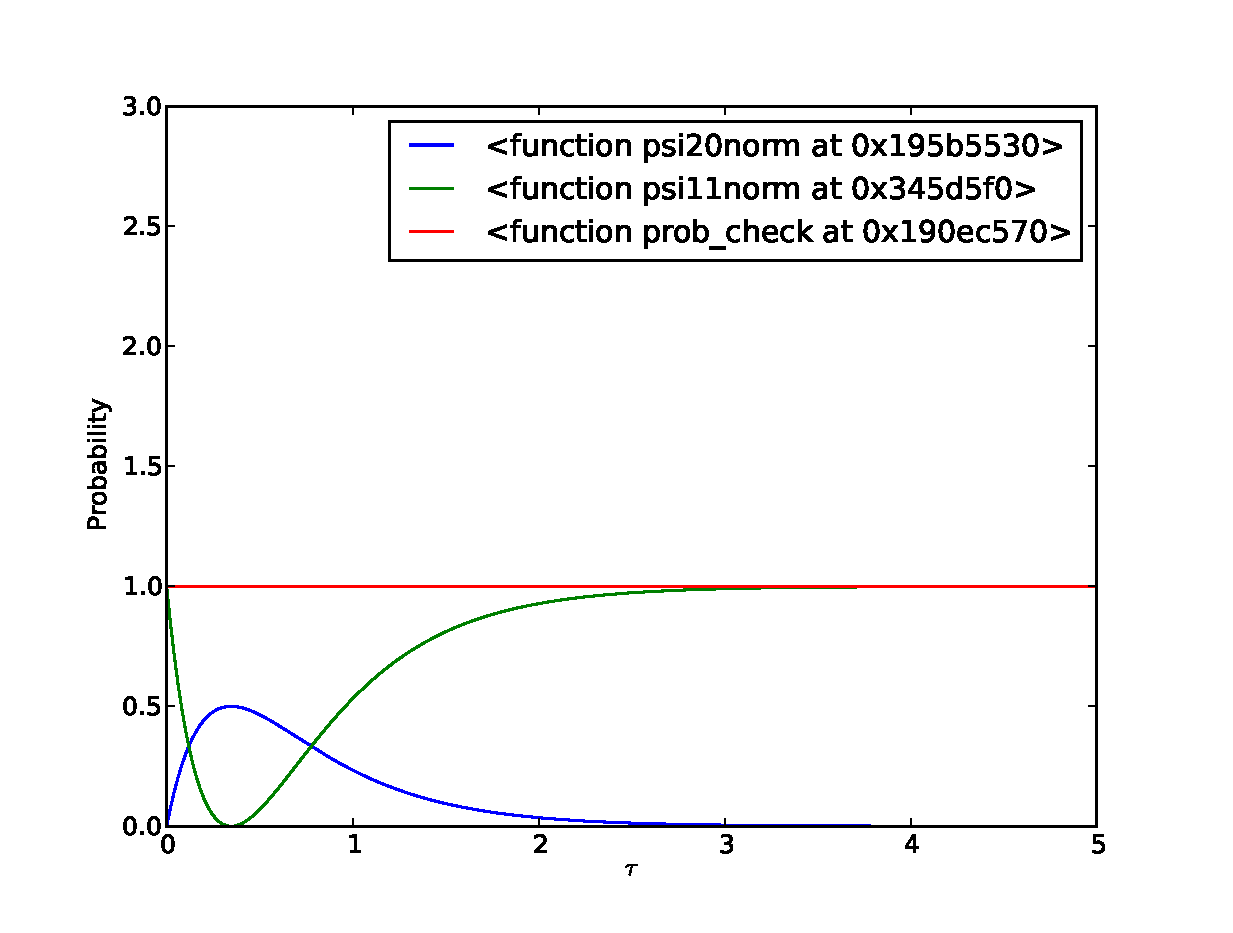
\epsfig{file=goodgraph.eps,width=1. \columnwidth}
\caption{The function prob-check sums up all the probabilities. Note: the function psi20norm is equal to psi02norm, so I only show one of them. Also psi20norm is the normalize function $|\langle \psi_20 | \Psi \rangle|^2$}

\end{figure}

However, if we plot the same functions vs the efficiency, the graph of the probabilities becomes:
\begin{figure}[H]
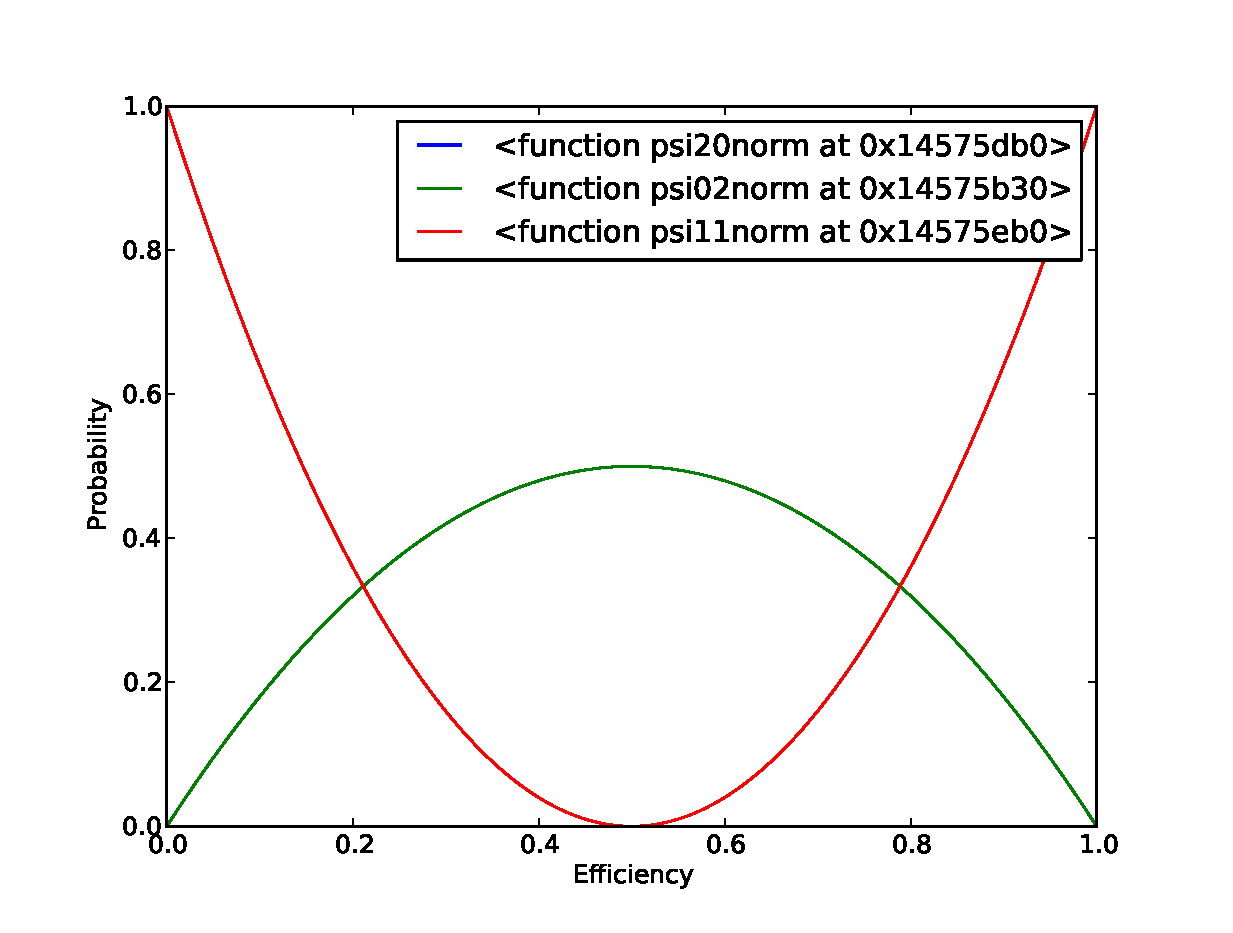
\epsfig{file=bsequiv.eps,width=.8 \columnwidth}
\caption{The same functions, plotted as a function of the efficiency of the system. Intuitively, we can interpret the efficiency as equivalent to the transmission co-efficient of the beamsplitter equations, as it is a measure of how much a single photon will come out of the system into the other 'mode' (atom-to-photon or photon-to-atom (atom-to-photon or photon-to-atom)). In this paradigm, the transmission co-efficient would be a measure of how much a single photon was converted into an atomic excitation}

\end{figure}

The equations that define the beamsplitter system can be solved to obtain:
\begin{align}
U_{BS} a U^\dagger_{BS} &= a_{out}= a \cos  |\theta| + b \sin| \theta|\\
U_{BS} b U^\dagger_{BS} &= b_{out}=b \cos  |\theta| - a \sin| \theta|
\end{align}
Where $a$ is the destruction operator for a mode. In the CD memory, we can think of this as a destruction operator acting on the photon field. Then $b$ is the destruction operator acting on the other mode coming into the beamsplitter. In the CD case, this would act on the atomic ensemble. Note, in this case we are in the Schrodinger picture, which is why we are looking at the dynamics corresponding to the unitary operator $U_{BS}$.


Now, if we find the probability of a state $\langle psi_{20} | =\frac{1}{\sqrt{2}} a^\dagger_{out} a^\dagger_{out} | 0 \rangle$, after preparing an initial state $| \Psi_11 \rangle = a^\dagger b^\dagger \rangle $ this is equal to:
\begin{align}
\langle \psi_{20}|\Psi_{11} \rangle = \sqrt{2} \cos |\theta| \sin |\theta|
\end{align}

However, using the equation for the transmission coefficient: 
$T = \cos|\theta|$, we can recast this equation into:

\begin{align}
\langle \psi_{20}|\Psi_{11} \rangle = \sqrt{2}  T\sqrt{(1-T^2)}
\end{align}
Square to get probability:
\begin{equation}
\label{bs20}
|\langle \psi_{20} | \Psi_{11} \rangle |^2 = T^2 (1-T^2) 
\end{equation}
And using a similar treatment, we can render the equation for the amplitude of a state $|\psi_{11} \rangle = a^\dagger_\textrm{out} b^\dagger_\textrm{out} | 0 \rangle$
\begin{align}
\langle \psi_{11} | \Psi_{11} \rangle &= \langle 0 | a^\dagger_{out}b^\dagger_{out} a^\dagger b^\dagger |0\rangle\\
&= \cos^2|\theta| - \sin^2|\theta|\\
&= -1+2T^2
\end{align}

and then square to get the probability:
\begin{equation}
|\langle \psi_{11} | \Psi_{11} \rangle |^2 = |-1+2T^2|^2 
\end{equation}
If we graph these equations, we can see that they are equivalent to the graph of the CD memory equations that were plotted as a function of the effiency.

\subsection{Mapping of CD to Beamsplitter}

If we take the equations derived that describe the dynamics of the CD-Memory in
the beamsplitter regime, Eqs. \eqref{p11},\eqref{p02},\eqref{p20}
and rewrite them in terms of the efficiency, $\eta$, we can see a full analytical
mapping between the equations for beamsplitters and the equations for CD.

Starting with a double excitation equation:
\begin{equation}
|\langle \psi_{20}| \Psi \rangle|^2=|A \sqrt{2} i(1- e^{-2\tau_w})
\end{equation}

We also know that the efficiency $\eta$, is equal to:
\begin{equation}
\eta = 1-e^{-2\tau_w}
\end{equation}
Additionally, we know that our normalization constant, A is:
\begin{equation}
A = \sqrt{\frac{1}{\left(  e^{2\tau_w} -1\right)}}
\end{equation}

And this can be rewritten in terms of $eta$ in the following way:
\begin{align}
A &= \sqrt{\frac{e^{-2\tau_w}}{1-e^{-2\tau_w}}}\\
A &=\sqrt{ \frac{1-\eta}{\eta}}
\end{align}

And rewriting Eq~\eqref{p20} in the same we, we obtain:
\begin{align}
|\langle \psi_{20}| \Psi \rangle|^2&= |A  \sqrt{2} i (1-e^{-2\tau})|^2\\
&=| \sqrt{\frac{1-\eta}{\eta}} \sqrt{2} \eta|^2\\ 
&= |  \sqrt{2} i \sqrt{ \eta (1-\eta)}|^2
\end{align}

We make the connection between the transmission coefficient and the efficiency by noting that:
\[
T^2 = \eta
\]
as $T^2$ will deal with the intensity of the field going through the beamsplitter, which is the analogy of how much of the atomic (photon) field is converted into the photon (atomic): this is what the efficiency measures.

Thus, the equation becomes:
\begin{align}
|\langle \psi_{20} | \Psi \rangle|^2 = | \sqrt{2} T\sqrt{1-T^2}|^2 \\
&= 2T^2 (1-T^2)
\end{align}
which, as we have shown earlier is the beamsplitter equation, exactly.

Similarly, we can show the equivalence between the $\langle \psi_{11} | \Psi \rangle$ states in the beamsplitter picture and the CD memory.
\begin{align}
\left | \langle \psi_{11} | \Phi \rangle \right | ^2  &= A^2\int^{t'} dt \left|\sqrt{\frac{2}{\kappa}} g(t) e^{-\tau(t)} \left (- e^{\tau(t')} +2 e^{-\tau(t')} \right ) \right |^2 \\
&= \frac{e^{-2\tau_w}}{1-e^{-2\tau_w}} \left (1- e^{-2\tau_w} \right ) \left ( e^{tau_w}-2e^{-\tau_w} \right )^2\\
&=  \left( 1-2e^{-2\tau_w} \right )^2\\
&= \left ( -1+2*\eta \right )^2\\
&= \left (-1+2*T^2 \right )^2
\end{align}

\section{AFC}

The afc memory has some differences from the CD-Memory, but it is also equivalent to a beamsplitter. Instead of the two channels being a memory storage and an emitted photon, you can think of the two channels as being two photons, but time delayed.

The section is laid out as follows:
\begin{description}
\item[ Section \ref{eqmot}]: I lay out the equations of motion
\item[ Section \ref{description}]: A high-level description of what is happening
\item [Section \ref{eqderv}]: A walk through of the calculations for the beamsplitting process.
\item [Section \ref{general}]: A presentation of the general case, where I plot the probabilites of the three states as a 
function of the efficiency/
\end{description}

\subsection{Equations of Motion}
\label{eqmot}
The equations of motion for the AFC memory in a cavity are:
\begin{align}
\dot{\sigma}_\omega (t) &= -i \omega \sigma - \gamma_h \sigma + i P E \\
\dot{E} (t) & = -\kappa E +\sqrt{2 \kappa} E_{in} + i \tilde{P} \int d \omega n(\omega) \sigma_\omega \\
E_{out} &= -E_{in} + \sqrt{2 \kappa} E
\end{align}

We can easily solve the equation for sigma, and then inserting it into the equation for
the cavity field. If we additionaly make the leaky cavity assumption, we can set $\dot{E} = 0$, and
and we have a solution for E, given by:
\begin{equation}
0 = -\kappa E +\sqrt{2 \kappa} E_{in} + i P \tilde{P} \int dt' \tilde{n} (t-t') E(t')
\end{equation}

You can see the AFC paper for more details, but because of the nature of the frequency
comb, the function $\tilde{n}(t-t')$ can be approximated by a chain of delta functions,
which are spaced apart by $\frac{2 \pi}{\Delta}$ in time.

Because of this, we can solve for local solutions for $E$ around peaks in the comb. In fact,
because the integral is over all time, we need to use a recursive strategy to solve
for the $E$ field at later times. This is because the $E$ field at some time $t \approx n\frac{2\pi}{\Delta}$ will depend
	on every previous $E$ field, due to the integral term $ i P\tilde{P} \int^t_{-\infty} \tilde{n}(t-t') E(t') d t'$


\subsection{High-Level}
\label{description}
The protocol works in the following way. There is an AFC memory in a cavity. The cavity has a decay rate of $\kappa$ that can be changed somehow. There is a pulse of light sent in with a time-envelope of $\Theta(t)$, such that is incident
upon the cavity at around $t~0$. Because of assumptions made in the AFC cavity protocol, the incident light pulse will
overlap with a narrow gaussian function, that can be approximated as a delta function. We additionally assume that the
impedence matching condition is on, such that $\kappa = \Gamma$, where $\Gamma$ is the absorption rate for the atoms within the gaussian spectral density. It has been shown that this can result in arbitrary close to unity efficiency. 

This means that there is one pulse now stored in the medium. Each 'tooth', or narrow gaussian function within the atomic
frequency comb will gain phase at different rates. However, because of the periodicity of the comb, each 'tooth' will
be in phase at $t = \frac{2 \pi}{\Delta}$. This means that the AFC is primed to re-emit at that time. 

However, right when the AFC is going to re-emit, we send in a second pulse of light, with time-envelope $\Phi$. Additionally, we change the cavity decay rate $\kappa$, such that the emission efficiency is $50\%$. This results in an interference
effect that I will show results in a $\frac{1}{2}$ probability of seeing two photons at that time.

If, however, we don't observe the photons at that time, we know that they must have both been stored in the cavity. We wait an additional rephasing has occured at time $t = \frac{4\pi}{\Delta}$ time, and change the emission efficiency back to $100\%$ by setting $\kappa = \Gamma$. In this way, we 'flush out' the memory. The equations show that there is a $\frac{1}{2}$ chance of seeing two photons there.

Additionally, I will also show that there is a zero chance of first seeing a photon at $t = \frac{2 \pi}{\Delta}$ and then seeing an additional photon at time $t = \frac{4 \pi}{\Delta}$.

A rough equivalence can be made to a physical beam splitter system, with two channels $a$ and $b$. If we have a time delay setup for any photons coming out in channel $b$, such that we introduce a delay of $\frac{2 \pi}{\Delta}$, and then
we recombine the photons. If we have a photon detector set-up, we will still be able to see photon bunching. There will be a 1/2 chance of seeing two photons in channel $a$, which will arrive at the photon detector at some time $t_1$. There will also be a 1/2 chance of seeing two photons in channel $b$, which will arrive later at some time $t_1+\frac{2 \pi}{\Delta}$. 
\subsection{AFC Photon Bunching}
This subsection is laid out as follows. I will first define the initial state, as there are some sublities involved. Then, I will prove that the initial state will only allow certain terms in any expansion of the oppurators of interest. Then, I will show the equations for each of the three states:
\begin{enumerate}
\item | $\langle \psi_{20} | \Psi \rangle |^2$, two photons detected around $t~\frac{2\pi}{\Deta}$
\item $ | \langle \psi_{02} | \Psi \rangle |^2 $, two photons detected around $t ~\frac{4 \pi}{\Delta}$
\item $ | \langle \psi_{11} |\Psi \rangle |^2 $, one photon detected around $t~\frac{2\pi}{\Delta}$ and one photon 
detected around $t~\frac{4\pi}{\Delta}$

\subsubsection{Initial State}
Note: This is a pedantic section, and it is fairly dull. You can skip over it, as it isn't that important. I just define the initial state, and then show a couple of specific results that I will reference later.

We first have to define the initial state. As previously laid out in the overview, we have two photons, one coming in
after the other, with time envelopes $\Theta$ and $\Phi$, respectively. Additionally, the two pulses are seperated by a time $\frac{2 \pi}{\Delta}$. I believe that we can define our initial state like:

\begin{align}
| \Psi \rangle &= \int d t' \int dt \Theta(t') E^\dagger_{in}(t') \Phi (t) E^\dagger_{in}(t)
\end{align}

Because the two pulses are far apart, we don't need to include a normalization factor of $\frac{1}{\sqrt{2}}$.

$E^\dagger_{in}(t)$ will create a photon incident on the cavity at some time $t$. The probability of this is weighted by
the envelope function, $\Theta$ or $\Phi$.

If we try to find the probability of seeing two photons exiting the cavity at some time $t$, we find the overlap between the two states:

\begin{equation}
| \rangle 0 | \frac{1}{sqrt{2}} E_{out}(t) E_{out}(t') |Psi |rangle |^2
\end{equation}

where $E_out$ is a heisenburg operator.

I am going to use a simplified equation for $E_{out}$ in order to prove that only cross terms will survive the expansion. This also lets me elaborate on the notation.

Assume that $E_{out}i(t) = a E_in(t) + b E_in(t-\frac{2\pi}{\Delta})$. 

Then, our probability for seeing two photons is at some time $t$ and $t'$:
\begin{align}
P2 = | \rangle 0 | \frac{1}{sqrt{2}} i(a^2 E_{in}(t) E_{in}(t') + b^2 E_in(t-\frac{2\pi}{\Delta}) E_in(t'-\frac{2\pi}{\Delta}) + ab E_{in}(t)E_in(t'-\frac{2\pi}{\Delta}) + abE_in(t-\frac{2\pi}{\Delta})E_{in}(t) ) |\Psi \rangle |^2 
\end{align}

If we look at the $a^2$ term, we can see that it won't survive when applied to the initial state.

\begin{align}
P2_1 =\langle 0 | a^2E_{in}(t) E_{in}(t') \int d t' \int dt \Theta (t') E^\dagger_{in}(t'') \Phi (t) E^\dagger_{in}(t''') | 0\rangle
\end{align}

Earlier, when the input-output equations were derived, there was a communtation relation, defined as:
\[
[E_{in}(t), E^dagger_{in}(t')] = \delta(t-t')
\]

Now, we know that any creation operator acting on a vacuum state like $\langle 0 | a^\dagger = 0$, so we can use
the commutation relations to 'shuffle' a creation operator to the very left, where it will destroy the vacuum. 

Therefore, P2 becomes:
\begin{align}
P2_1 &=  \langle 0 |\int dt'' \int dt'''\Theta(t'')\Phi(t''') a^2 E_{in}(t)(E^\dagger_{in}(t'')E_{in}(t') +\delta(t'-t'') ) E\dagger_{in}(t''') |0|rangle\\
& = \langle 0 | \int dt'' \int dt''' \Theta(t'') \Phi(t''') a^2 (E^\dagger_{in}(t'')E_{in}(t)+\delta(t-t''))E_{in}(t')E\dagger_{in}(t''')
+ E_{in}(t)\delta(t'-t'')E^\dagger_{in}(t''') \\
&= \langle 0 |\int dt'' \int dt''' \Theta(t'') \Phi(t''') a^2 ( 0 + \delta(t-t'') (E^\dagger_{in}(t''')E_{in}(t') + \delta(t'-t''') ) + E_{in}(t)\delta(t'-t'')E^\dagger_{in}(t''')|0\rangle
&= \int dt'' \int dt'''\Theta(t'')\Phi(t''') a^2(\delta(t-t'')\delta(t'-t''')+\delta(t'-t'')\delta(t-t''')
&= a^2\Theta(t)\Phi(t')+a^2\Theta(t')\Phi(t)
\end{align}

So, in order to be more general, we would integrate this term over the local time of one of the teeth. More specifically, we would integrate this probability equation all over the areas where the equation is valid-- this is constrained to times $t~\frac{2 \pi}{\Delta}$. However, because we are integrating both $t$ and $t'$ at around the same values, the P2_1 term is zero, as we know that there is a time delay between both pulses. This is a subtle point, and I am not explaining it well. In order for the P2_1 term to have been valid, it would have needed something like:
\begin{align}
P2_1 = a^2 \Theta(t-\frac{2\pi}{\Delta})\Phi(t') +a^2\Theta(t'-\frac{2\pi}{\Delta})\Phi(t)
\end{align}

So that even though \Theta and \Phi don't overlap, the above function will evaluate to some non-zero. This only comes through in the cross terms.

In my future calculations, I will take it as given that we can drop the $a^2$ and the $b^2$ terms. Ie, everything but the cross terms.

\subsubsection{The Three States}
\label{sec:three}
In order to calculate the evolution of the states of interest, we first need to mathematically define our states of interest:
\begin{align}
\label{eq:p20}
P20(t,t') = | \langle 0 | \frac{1}{\sqrt{2}} E_{out}(t) E_{out}(t') | \Psi \rangle |^2
\end{align}

where $t~\frac{2\pi}{\Delta}$ and $t' ~\frac{1}{2 \pi}{\Delta}$
\begin{equation}
\label{eq:p11}
P11(t,t') = | \langle 0 | \frac{1}{\sqrt{2}} E_{out}(t) E_{out}(t') | \Psi \rangle |^2
\end{equation}
where $t~\frac{2\pi}{\Delta}$ and $t'~\frac{4 \pi}{\Delta}$

\begin{equation}
\label{eq:p02}
P02(t,t') = | \langle 0 | \frac{1}{\sqrt{2}} E_{out}(t) E_{out}(t') | \Psi \rangle |^2
\end{equation}
where $t~\frac{4\pi}{\Delta}$ and $t'~\frac{4\pi}{\Delta}$

So, the first deals with the probabilty of observing two photons around the neighborhood of $t~\frac{2 \pi}{\Delta}$, the second term deals with first observing a photon in the neighborhood of $t~\frac{2 \pi}{\Delta}$ and then observing a photon in the neighborhood of $t~\frac{4 \pi}{\Delta}$, and the third term deals with observing two photons in the neighborhood
of $t~\frac{4 \pi}{\Delta}$

\label{eqderv}
\subsection{Photon Bunching}
\label{phbnch}

In this section, I will deal with each of the probability terms defined in section \ref{sec:three}, and calculate them out. I will be dealing with the specific condition where the impedence matching condition is perfect for the very first pulse, and then set to 50\% efficiency for the second pulse.

\subsubsection{P20}
First, we must calculate what the $E_{out}$ operator is during this time. The physical situation is that we have a
pulse read in with near unit efficiency, but just as it is about to rephase, we send another pulse in. The general equation for $E_{out}$ is:
\begin{align}
E_{out} = \sqrt{2\kappa} - E_{in}
\end{align}

So we must first calculate what the cavity field $E$ is doing. The equation of motion for $E$ is given by:

\begin{align}
\dot{E} = -\kappa E -iP\tilde{P}\int_{-infty}^t\tilde{n}(t-t')E(t')+\sqrt{2\kappa} E_{in}(t)
\end{align}

We can divide the integral up into two segments. The first segment $-\infty<t\le0$ is where the first pulse is being read in with unit efficiency. In the impedence matching paper, this condition was already derived, and the equation for $E$ during this time is $E = \frac{1}{\sqrt{2\kappa}}$, with $\kappa = \Gamma$, where $\kappa$ is the cavity decay rate, and $\Gamma$ is the absorption by the atomic frequency comb. However, in order to simplfy the equations that will come later, in the unit efficiency case, I will be rewriting the equations to include $\Gamma$ instead of $\kappa$. I can do this
because of their equivalence, and it means that I won't have to worry about having different $\kappa$'s. This is because we will be changing the cavity decay rate, so $\kappa$ is not a constant in time. By renaming it to $\Gamma$, it will hopefully make the end equations more managable. So when ever you see a $\kappa$, you can assume it is a cavity decay rate that sets the absorption efficiency to 50\%.

So, the second sequence is when $t'~t$, and in that case, $E(t')$ is just $E(t')$, as it is in the neighborhood of the time
that we are evaluating at. Broken up this way, the equation becomes
\begin{align}
\dot{E} & = -\kappa E -2\Gamma \frac{1}{\sqrt{2\Gamma}}E_{in}(t-\frac{2 \pi}{\Delta}) -\Gamma E(t) +\sqrt{2 \kappa} E_{in}(t)
\end{align}

Using the usual trick of setting $\dot{E}=0$, we can solve for E:
\begin{equation}
E = \frac{\kappa +\Gamma} (\sqrt{2 \Gamma} E_{in}(t-\frac{2 \pi}{\Delta} +\sqrt{2 \kappa}E_{in}(t)
\end{equation}

So, using this equation in our equation for $E_{out}$, we get:

\begin{align}
E_{out} &= \frac{\sqrt{2\kappa}}{\kappa+\Gamma} (\sqrt{2 \Gamma} E_{in}(t- \frac{2 \pi}{\Delta} +\sqrt{2\kappa} E_{in}(t)_ - E_{in}(t)\\
&= \frac{2 \sqrt{\kappa \Gamma}}{\kappa + \Gamma}E_in(t- \frac{2\pi}{\Delta} +\frac{\kappa - \Gamma}{\kappa+\Gamma} E_{in}(t)
\end{align}



\subsection{AFC Photon Interference}
\label{general}


\section{Conclusion}

I have shown full analytical equivalence between the CD-memory in the two photon regime, and a beam-splitter.
\end{document}


